\section{Rosenbrock function}
\label{sec:rosenbrock_results}

We first test our implementation of the optimization algorithms on the Rosenbrock function, defined as follows.
\begin{equation}
    f(x) = 100(x_2 - x_1^2)^2 + (1 - x_1)^2
\end{equation}
The Rosenbrock function is a non-convex function that is commonly used to test optimization algorithms. It has a global minimum at $x^* = (1, 1)$, where $f(x^*) = 0$. The function is characterized by a narrow, curved valley, which makes it difficult for optimization algorithms to converge to the global minimum.
We test the algorithms on the Rosenbrock function with two different starting points: $x_0^{(1)} = (1.2, 1.2)$ and $x_0^{(2)} = (-1.2, 1)$. The results are shown in Figure~\ref{fig:rosenbrock}.
Both methods converge to the global minimum in both cases, but the Modified Newton method converges faster than the Truncated Newton method. The results are summarized in Table~\ref{tab:rosenbrock_results}.
\begin{itemize}
    \item For the starting point $x_0^{(1)} = (1.2, 1.2)$, the Modified Newton method converges in a number of iterations that is comparable to the Truncated Newton method: this is expected since the starting point is close to the minimum, so the Newton system is solved accurately.
    \item For the starting point $x_0^{(2)} = (-1.2, 1)$, the Modified Newton method converges in fewer iterations than the Truncated Newton method: this is expected since the starting point is far from the minimum, so the Newton system is solved approximately in the first steps: this lead to a very slow progress in the first iterations of the Truncated Newton method.
\end{itemize}
In both cases, despite the fact that the Truncated Newton method requires more iterations, its execution time is comparable or even lower than Modified Newton method.
This is due to the fact that the Truncated Newton method requires less computational effort per iteration.
\begin{table}
    \centering
    \begin{tabular}{c|c|c|c|c|c|c}
        \toprule
        Starting Point & Algorithm & Iterations & $\| \nabla f(x_k) \|$ & $f(x_k)$ & Time (s) & $x_k$ \\
        \midrule
        \multirow{2}{*}{$x_0^{(1)} = (1.2,\, 1.2)$} & Modified Newton & 8 & 1.436e-11 & 1.0883e-25 & 0.009753 & $(1.0000,\, 1.0000)$ \\
        & Truncated Newton & 9 & 1.0471e-07 & 5.5531e-18 & 0.010447 & $(0.9999,\, 0.9999)$ \\ \midrule
        \multirow{2}{*}{$x_0^{(2)} = (-1.2,\, 1)$} & Modified Newton & 21 & 4.4733e-10 & 3.744e-21 & 0.001906 & $(0.9999,\, 0.9999)$ \\
        & Truncated Newton & 64 & 9.1038e-15 & 2.072e-29 & 0.00128 & $(0.9999,\, 0.9999)$\\
        \bottomrule
    \end{tabular}
    \caption{Results of optimization algorithms on the Rosenbrock function with different starting points.}
    \label{tab:rosenbrock_results}
\end{table}

\begin{figure}
    \centering
    \begin{subfigure}{0.49\textwidth}
        \centering
        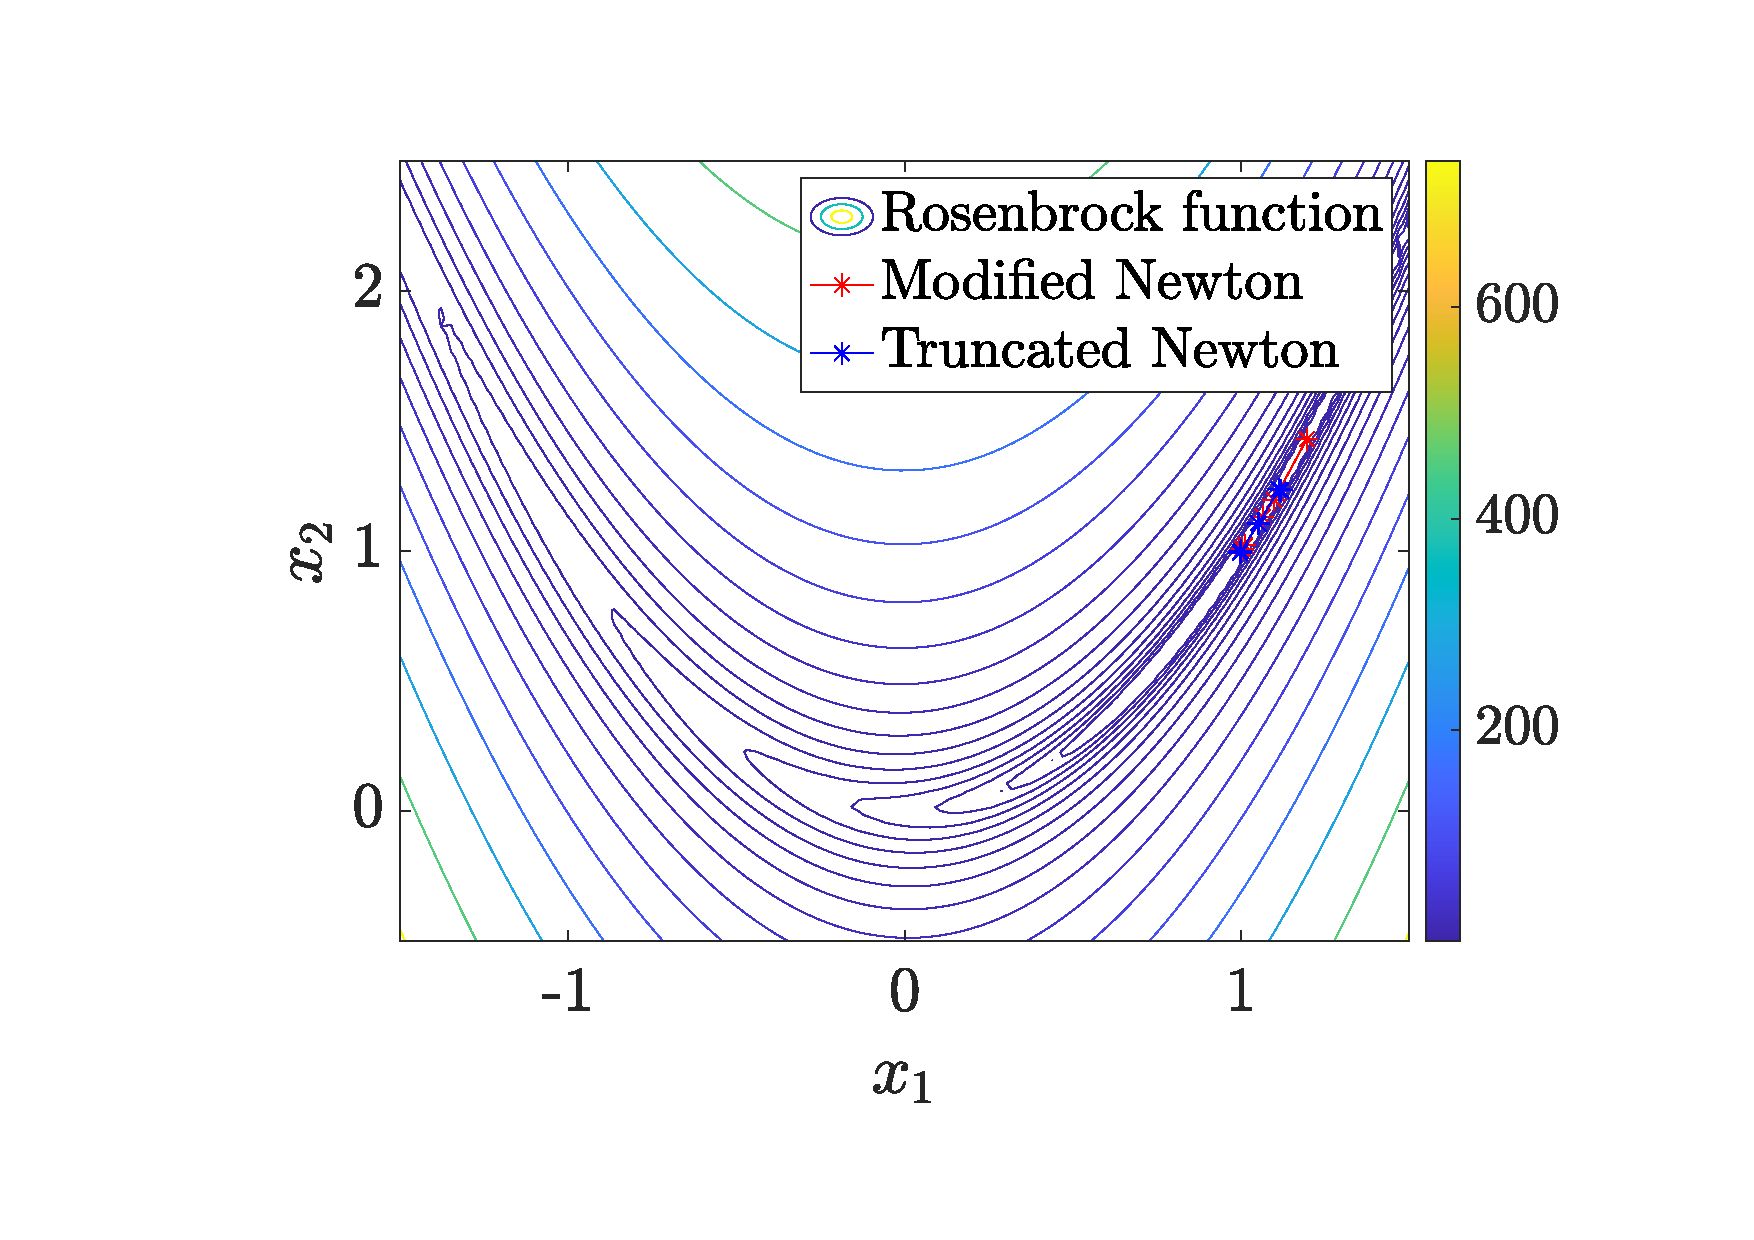
\includegraphics[width=\linewidth]{figures/rosenbrock_x0_1.pdf}
        \label{fig:rosenbrock_x0_0}
        \caption{Starting point $x_0^{(1)} = (1.2, 1.2)$}
    \end{subfigure}
    \begin{subfigure}{0.49\textwidth}
        \centering
        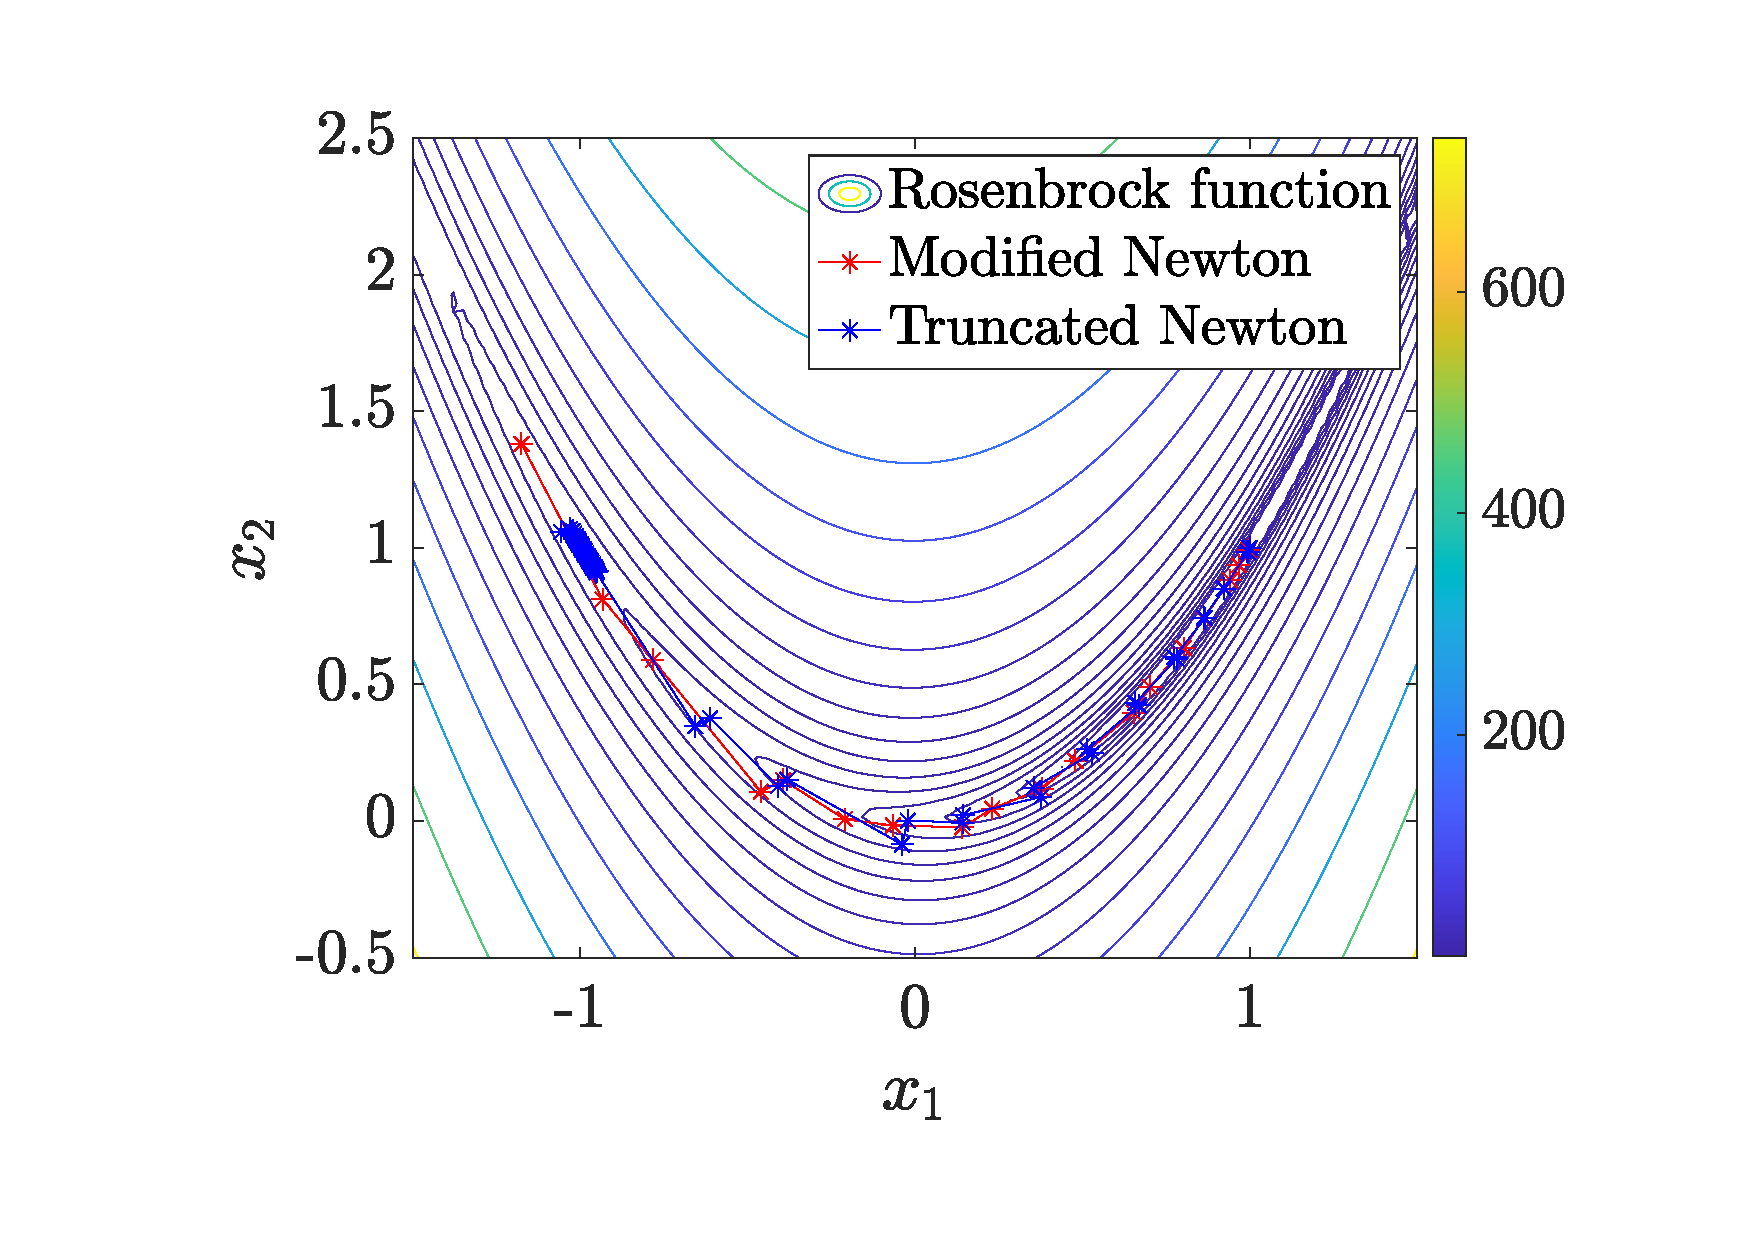
\includegraphics[width=\linewidth]{figures/rosenbrock_x0_2.pdf}
        \label{fig:rosenbrock_x0_1}
        \caption{Starting point $x_0^{(2)} = (-1.2, 1)$}
    \end{subfigure}
    \caption{Convergence of the algorithms on the Rosenbrock function with different starting points and different optimization algorithms.}
    \label{fig:rosenbrock}
\end{figure}